\documentclass[12pt]{unlsilabsop}
\title{Visual inspection of HDI}
\date{April 23, 2015}
\author{Frank Meier Aeschbacher}
\approved{Frank Meier Aeschbacher}
\sopid{201}
\sopversion{v1}
\sopabstract{Describes the procedures for visual inspection of HDI. This consists mainly of an inspection by eye and using a microscope. Any deviations from normal appearance will be documented.}
\begin{document}

\maketitle

%------------------------------------------------------------------
\section{Scope}
This is a regular test in the manufacturing process of pixel modules at UNL.

%------------------------------------------------------------------
\section{Purpose}
HDI are a critical part for manufacturing modules. This test is a critical control point to make sure the material we receive meets expectations and to ensure the quality of our modules built out of it.

%------------------------------------------------------------------
%>\section{Definitions}

%------------------------------------------------------------------
%\section{Responsibilities}

%------------------------------------------------------------------
\section{Equipment}

\begin{itemize}
\item \textbf{Probe station} Jmicro JR-2745, to hold the setup
\item \textbf{Microscope with camera and LED ring illumination} Microscope at probe station, with camera connected to the computer
\item \textbf{Gooseneck LED lamps} mounted on microscope stand
\item \textbf{Computer} Requires ToupeViewX installed (software to grab images from microscope camera) and ImageMagick
\end{itemize}

%------------------------------------------------------------------
\section{Procedure}

\begin{enumerate}
    \item Handle HDI only with proper protection: ESD wristband, gloves, face mask.
    \item Take note of identifying information printed on the HDI: work order, manufacturing week and year, panel and position numbers. Record.

    \begin{center}
        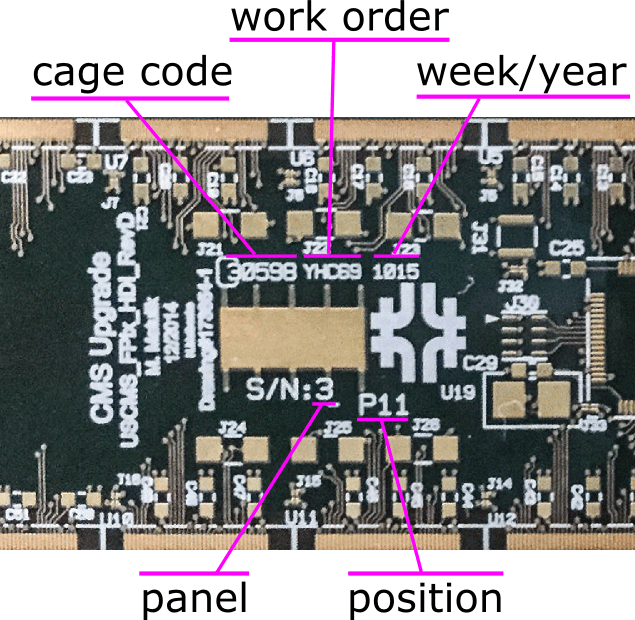
\includegraphics[width=7cm]{img/HDIRevD_id.png}
    \end{center}

    \item Remove HDI from its container and place on probe station. You can hold HDI at the end holders with your fingers or use tweezers. Do not touch any other parts of the HDI.
    \item Start up camera software on computer
    \item Starting on the top left corner, zoom in with microscope until the field of vision from left to right is approximately the width of one ROC (=group of 35 bond pads).
    \item Move the table using the knob. Scan both long edges of the HDI and check for any obvious damage or dirt.
    \item Move to the center where the TBM chip is mounted. Check if the wirebonds are ok.
    \item Move to the neighboring wirebonds that set the module address. There should be four bonds in good shape.
    \item Document any findings. Any damage visibile or unusual feature needs to be documented using a picture. Adjust the exposure in a way to capture bright and dark areas at the same time. If needed, adjust lighting conditions. The controller for the LED ring allows to adjust the brightness and switch quadrants on and off. Label files with a clear ereference to the module and the position this image shows.
\end{enumerate}
\textbf{Note:} The image capturing software only allows to store bitmap files (\texttt{*.bmp}), which are too large to be stored in the database or the elog. To convert files, use ImageMagick from the command line as follows:

\medskip

\texttt{\$> convert -resize 1024x768 filename.\{bmp,jpg\}} 
\medskip

where \texttt{filename.bmp} is the name of the file given when the image got saved in the camera capture software.

%------------------------------------------------------------------
\section{Documentation}
Status of the HDI needs to be updated in the Purdue database. Go to ``MAIN MENU''$\rightarrow$``Part List'' and select your HDI. Upload any pictures as needed and add comments as needed. Check the tickmark on ``Inspected'' and hit ``SUBMIT''. 

No need to make an entry in the Elog if nothing special happened.

\end{document}

